\documentclass[a4paper,twoside]{article}
\usepackage[T1]{fontenc}
\usepackage{graphicx}
\usepackage{calc}
\usepackage{amssymb}
\usepackage{amsmath}
\usepackage{pslatex}
\usepackage{apalike}
\usepackage{booktabs}
\usepackage{algorithm2e}
\usepackage[bottom]{footmisc}
\usepackage[hidelinks,breaklinks]{hyperref}
\usepackage{SCITEPRESS}
\hypersetup{pdftitle={From Candidate Coverage to Correct Plans: A Position on LLM Planning Evaluation},pdfauthor={},pdfsubject={Anonymous position paper},pdfkeywords={LLM Planning, Semantic Validation, Evaluation},pdfcreator={LaTeX}}

\begin{document}
\title{From Candidate Coverage to Correct Plans: A Position on LLM Planning Evaluation}
\author{}
\keywords{LLM Planning, Semantic Validation, Candidate Coverage, Decision Correctness, Evaluation.}
\abstract{A solver can correctly solve an incorrectly formalized request. Evaluating the resulting plan alone does not reveal whether failure arose from an uninformative benchmark, missing interpretations, ineffective validation, or unreliable selection. We argue that evaluations of language-model planning should connect four measurements: requirement coverage in the planning universe, availability of a reference-matching interpretation, consequential distinguishability, and conversion into correct decisions, with inference cost reported alongside them. Two exploratory studies of constructed transit requests grounded in published schedules motivate this position. In 48 requests, consequence-weighted validation changed witness sequences in only two cases and tied balanced selection at 33 correct outcomes. In a separate 32-request study, diversified sampling increased bounded candidate coverage from 27 to 31 requests relative to independent sampling, while both produced 28 correct final outcomes. Solver-guided sampling achieved 25 on both measures at greater token cost. Joint request-level analysis exposes failures despite available matching candidates and success without a matching formalization. These findings support a diagnostic reporting procedure, not an advantage for either proposed intervention. Small samples, provisional annotations, one model, and bounded bus-only universes limit the empirical claims.}
\onecolumn \maketitle \normalsize \setcounter{footnote}{0} \vfill

\section{\uppercase{Position and Context}}
\label{sec:position}
\noindent A language model can turn a request into constraints that a solver satisfies exactly, yet misrepresent the request. An upper departure bound can become a lower bound, making the solver optimize the wrong feasible set without a computational error.

We argue for connecting four questions: does the benchmark exercise the intended requirements; is a matching interpretation available; can validation distinguish consequential alternatives; and does selection convert available interpretations into correct decisions? Joint request-level measurements and inference costs complement aggregate accuracy.\footnote{OpenAI Codex assisted prose throughout and offline analysis/figure code \cite{codex}; the disclosure following Section~\ref{sec:conclusion} specifies its scope.}

The position arose through two exploratory civilian transit studies: consequence-weighted example selection and solver-guided candidate sampling. Neither improved final correctness over its principal baselines. Their negative findings expose limited opportunity to act, candidate coverage that fails to reach the final decision, and feedback that adds cost without useful exploration.

The contribution is a concrete reporting procedure linking these observations. Its measurements and probability identities are elementary. We claim no novelty for model--solver combinations, repeated sampling, diverse prompts, semantic equivalence, or distinguishing examples, and no general failure of those techniques.

\subsection{What Closest Work Already Measures}

Formalization quality is an established concern. Comparisons of models as formalizers and solvers on constraint-satisfaction tasks identify a translation bottleneck \cite{amonkar}. Our focus is the subsequent relationship between executable candidate sets and selected decisions.

Semantic Self-Verification (SSV) uses concrete instantiations to check and repair formalizations and reports accuracy, verification precision, and verification coverage \cite{ssv}. Its coverage is the proportion receiving verification; ours measures whether a candidate set contains a reference-matching behavior. Separating coverage and accuracy is a precedent. We extend their diagnostic relationship to the availability and correctness of planning decisions.

ARTEMIS supports semantic validation through low-complexity distinguishing traces, assessing accuracy and validation effort \cite{artemis}. Our balanced selector adapts this idea to finite journey pools and model judgments; it does not reproduce human-assisted ARTEMIS. Our same-model judge results cannot directly refute human-validation findings.

Sampling-diversity research already distinguishes generating a correct solution from selecting it, including limits of majority voting \cite{diversity}. We instantiate that concern with journey acceptance vectors and both off-diagonal outcomes: losing a matching candidate and producing a correct plan without one.

VERGE combines equivalence-based consensus, semantic alignment, solver feedback, and routing, and reports a formalization funnel, failure modes, and matched-token comparisons \cite{verge}. Component diagnosis and compute accounting are not unique to our proposal. Our extension links independently evaluated candidate availability to final decisions on the same requests while auditing whether the benchmark supplies meaningful semantic distinctions.

\section{\uppercase{An Evaluation Procedure}}
\label{sec:framework}
\noindent Let $x$ be a request and $J_x$ its finite planning universe, constructed from published schedules and public scenario metadata. Each valid candidate interpretation $C$ maps journeys to Boolean acceptance. Let $R_x$ denote a separately specified reference evaluator. The behavioral signature is
\begin{equation}
  \sigma_{J_x}(C)=(C(j))_{j\in J_x}.
\end{equation}
Equality of signatures establishes equivalence only within $J_x$. It proves neither unrestricted logical equivalence nor correspondence to every aspect of the natural-language intent. In particular, an uninformative universe can make different meanings behaviorally identical. References may also be wrong; their annotation provenance must remain visible.

\subsection{Availability and Final Correctness}

For the valid candidates $\mathcal{C}_x$ available at a frozen checkpoint, define
\begin{equation}
 G_x=\mathbf{1}\{\exists C\in\mathcal{C}_x:
                 \sigma_{J_x}(C)=\sigma_{J_x}(R_x)\}.
\end{equation}
Let $S_x=1$ when the final output is either a journey satisfying $R_x$ or a correct conclusion that no journey in $J_x$ satisfies it. A timeout, malformed output, abstention, or false infeasibility claim is not a correct resolution. These categories should also be reported separately so that a method cannot appear better merely by returning fewer plans.

The joint cells distinguish conversion $(1,1)$, loss despite availability $(1,0)$, success without a match $(0,1)$, and failure without one $(0,0)$. The ordinary probability decomposition
\begin{align}
 P(S=1)={}&P(G=1)P(S=1\mid G=1)\nonumber\\
          &+P(G=0)P(S=1\mid G=0)
\end{align}
organizes these observations; it is not a new theorem. Marginal coverage and correctness do not determine the joint table. A formalization may accept some wrong journeys while its selected journey satisfies the request. Such a success need not be dismissed as accidental, but it cannot certify the whole formalization.

For each $(1,0)$ case, trace the actual loss: a wrong judgment, tie-breaking, budget exhaustion, or an update removing a useful candidate. Availability alone does not identify the cause. Likewise, $(0,0)$ does not establish that every candidate-selected plan was wrong; their particular outputs must be checked.

\subsection{Consequential Distinguishability}

Let $\pi_i$ be the deterministic plan selected under candidate $C_i$. A journey distinguishes $i$ and $j$ when their acceptance values differ. We used the consequence indicator
\begin{equation}
 I_{ij}=\mathbf{1}\{\neg C_j(\pi_i)\}
       +\mathbf{1}\{\neg C_i(\pi_j)\},
\end{equation}
where a missing plan contributes zero to its term. This convention handles an infeasible interpretation without inventing a plan. The score describes cross-interpretation incompatibility, not which interpretation is correct.

The balanced score sums one over separated pairs and divides by positive witness cost; the weighted score substitutes $1+I_{ij}$. With uniform positive pair weights, shared costs, and shared tie-breaking, one objective is a positive scalar multiple of the other: rankings are identical. Two candidates have only one pair. Identical sequences additionally require identical judgments and updates at shared states. This explains these implemented objectives, not every consequence-sensitive method.

\subsection{Coverage Before Interpretation}

A requirement appearing in a request does not establish that the pool tests it. Record whether each reference clause accepts some journeys and rejects others. Then check conditional relevance: can it exclude a journey satisfying the other clauses? This distinguishes informative requirements from constant or masked restrictions.

Stronger contrasts may be necessary. Testing ordered visits requires distinguishing the requested order from another order while holding stop presence fixed. Variation in ``visit these stops in this order'' alone does not demonstrate order sensitivity. Coverage is family-specific; truth-vector variation is a minimum, not a complete semantic audit.

\section{\uppercase{Two Exploratory Transit Studies}}
\label{sec:setup}
\noindent Both studies use constructed requests grounded in a frozen September 2026 TriMet GTFS feed \cite{trimet,gtfs}, not passenger records or observed movements. Service is evaluated on 14 September 2026 in \texttt{America/Los\_Angeles}, with calendars, exceptions, service-day seconds, and inclusive request boundaries. Daytime scenarios do not exercise the parser's beyond-midnight support.

A pre-output coverage rule selected connected bus routes 2, 4, and 17 in downtown Portland. Journeys have at most two rides per segment and exact-stop transfers with a 120-second minimum. Walking, through-service, capacity, and accessibility guarantees are excluded. Public endpoints and horizons define the universe; references and predictions never prune it. Plans optimize arrival, boardings, departure, then journey ID. Enumeration caps make every feasibility and equivalence claim pool-relative.

The typed language supports time bounds, transfers, modes, scoped segments, ordered visits, and Boolean composition. A deterministic compiler interfaces with Z3, while separate reference code evaluates outcomes. Model-generated Python is not executed. Exact and behavioral duplicates are removed; raw attempts remain preserved. Selection retains the first surviving candidate in generation order, without reference guidance.

\subsection{Shared Model and Validation}

Both use Qwen2.5-7B-Instruct \cite{qwen}, revision \texttt{a09a35458c702b33eeac\allowbreak{}c393d103063234e8bc28}, BF16, Transformers 4.51.3, and PyTorch 2.8.0/CUDA 12.8. Sampling uses temperature 0.7, top-$p$ 0.95, top-$k$ 20, repetition penalty 1.05, and at most 768 output tokens. Each base has one replicate.

The ordinary judge receives only the original request and a deterministic journey description with times, stops, and transfers. Candidate formulas, votes, reference labels, and selector preference are hidden. It returns satisfied, violated, or uncertain; definitive labels eliminate inconsistent candidates. Translation and judgment use the same model in fresh invocations, not an independent truth oracle. Principal comparisons use elimination only, without repair-generated candidates.

References precede generation and remain separate from runtime inputs. Developer/automated checks found no clear correction in Study 1, but neither study has independent human adjudication. Raw outputs and frozen protocols support offline replay. This paper used no new experimental inference.

\subsection{Study 1: Selecting Validation Examples}

The selector study comprises 48 fresh base requests, one replicate each, using 07:00--10:00 schedules. Eight requests each target timing, transfers, mode exclusions, outbound/return scope, ordered visits, and infeasibility. Forty are reference-feasible and eight infeasible within their pools. The 48 pools contain 4,366 journey memberships, capped at 64 per single segment and 256 for combined journeys; 40 pools were truncated.

Each request supplies the same four raw candidate attempts to the balanced and consequence-weighted selectors. The witness cost is one. Budgets of zero, one, two, and four judgments reuse trajectory prefixes. The original target of two replicates was reduced to one by a frozen throughput rule before comparative evaluation. No candidate errors were deliberately injected into the experiment.

\subsection{Study 2: Sampling Interpretations}

The sampling study uses 32 new base requests and 10:00--13:00 schedules. Prior origin--destination groups and their reverses are excluded, but routes, stops, date, and templates overlap. This separate protocol is not an independent replication. Twenty-eight requests are feasible and four infeasible. Timing, transfer, and scope requirements were selected for informative contrasts; modes and ordered visits were omitted. All 56 reference clauses vary and have conditional exclusions. Pools retain at most 128 journeys per segment and 256 combined journeys.

Independent sampling repeats the base prompt. Diversified sampling adds frozen source-focused perspectives on timing and scope. Solver-guided sampling adds deterministic summaries of prior formulas, full/clause signatures, and concrete journeys to the same perspectives, explicitly permitting repeated readings. Feedback excludes references and ordinary judgments. Shared source-only time normalization corrects unambiguous values, but not missing constraints or wrong operators.

The first two samples are shared across arms. Full trajectories precede evaluation of two-, four-, and eight-attempt prefixes, each with balanced selection and at most two judgments. Identical allocations permit 35,000 generation tokens per request and 4,000 validation tokens per prefix, counting input plus output. Calls require enough allowance for their input and maximum output. No allowance was exhausted: eight attempts stopped every trajectory. These are equal ceilings, not equal actual compute.

\section{\uppercase{What the Studies Reveal}}
\label{sec:findings}
\noindent The following analyses use base requests as the observational unit. Stage-specific denominators remain separate. Candidate attempts, checkpoints, and reused judgments are not independent observations. The offline tables and figures were reconstructed from preserved outputs, including joint outcomes and privileged-label replay.\footnote{The reconstruction and plotting code were prepared with Codex assistance \cite{codex}; figures are deterministic plots of saved records, not generated illustrations.}

\subsection{Little Opportunity for Weighting}

In Study 1, 25 of 48 bundles contain distinguishable interpretations, and 18 contain consequential plan disagreements. These are nested sets, but consequence does not imply a change in witness ranking (Figure~\ref{fig:opportunity}). Fourteen of the 18 consequential bundles have uniform pair weights. Of the remaining four, two choose the same initial witness through shared tie-breaking and subsequently have at most two surviving classes. Only two requests have different witness sequences. Their correctness outcomes still agree; only one final plan identifier differs.

\begin{figure*}[t]
\centering
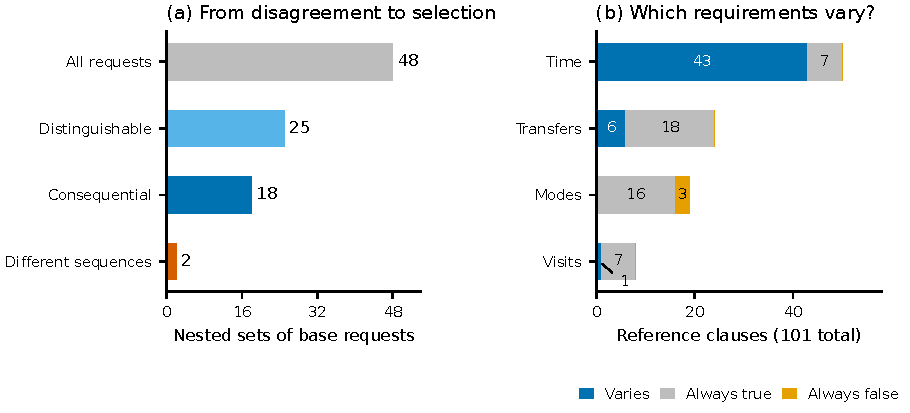
\includegraphics[width=\textwidth]{figures/selector-opportunity.pdf}
\caption{Study 1: opportunity for selector improvement and effective requirement coverage. Left: the nested sets contain 48 requests, 25 distinguishable bundles, 18 consequential bundles, and two divergent witness sequences. Fourteen consequential bundles have uniform weights; two more retain the same selection through tie-breaking. Right: truth variation of 101 reference clauses across their respective pools. All 19 mode clauses are constant. One of eight visit clauses varies, but none tests ordering beyond stop presence. Counts describe this bus-only benchmark, not general transport coverage.}
\label{fig:opportunity}
\end{figure*}

Both selectors resolve 31/48 requests at budget zero and 33/48 at budgets one, two, and four: three recoveries and one deterioration, a net 4.17-point gain. In the deteriorated case, a correct negative judgment removes a wrong formalization whose initial plan was valid. Reliable judging cannot prevent every loss when candidate coverage is inadequate.

Each selector returns 30/40 valid feasible plans, five invalid plans, and five false infeasibility conclusions. It identifies 3/8 infeasible requests; five give invalid interpretation outputs. No unresolved or infrastructure failures occur. Budget two adds four judgments per method but changes no plan; budget four adds no judgments. Exhausted distinctions explain the flat curve. Oracle-witness replay reaches 35/48 for both, without a weighting advantage.

The coverage audit also limits interpretation. Only 50/101 reference clauses vary across their pools; 48 are always satisfied and three always violated. Six of 24 transfer clauses vary, although 45/48 pools contain both zero- and one-transfer journeys. With at most two rides, an at-most-one-transfer clause is vacuous. All 19 mode clauses are constant. Ordered visits never exclude a journey beyond requiring both stops to be present. Removing enumeration caps increases memberships to 77,871 but adds no candidate classes or witness partitions for these saved bundles. The limitation is not simply too few enumerated paths.

\subsection{Coverage Gains Do Not Ensure Better Plans}

All Study 2 arms begin with 25/32 coverage and correctness. At eight attempts, independent sampling reaches 27/32 coverage and 28/32 correctness; diversified sampling reaches 31/32 and 28/32; solver-guided sampling stays at 25/32 on both (Figure~\ref{fig:cost}). Solver-guided sampling adds no matching behavior after the shared samples. Mean distinct full signatures are 1.41, 1.59, and 1.19, respectively: more feedback did not yield useful exploration.

\begin{figure*}[t]
\centering
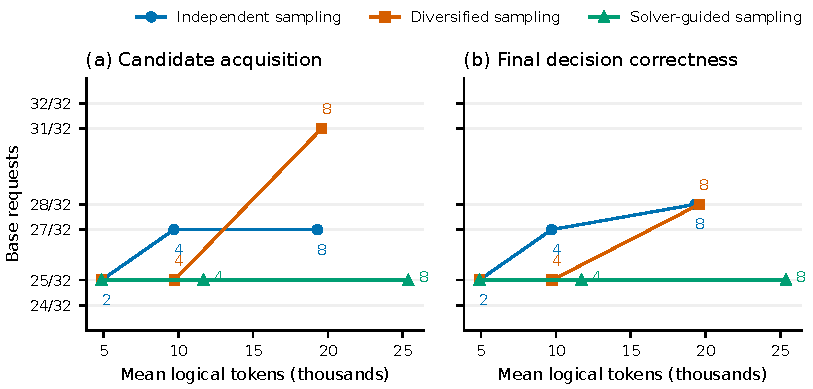
\includegraphics[width=\textwidth]{figures/cost-outcomes.pdf}
\caption{Study 2: candidate availability and ordinary final correctness at the frozen two-, four-, and eight-attempt checkpoints (point labels), each over 32 base requests. Horizontal positions are mean logically attributed input plus output tokens for candidate generation and validation of that prefix. Lines connect observed checkpoints only. The first two samples are shared. Equal allocations did not imply equal consumption; no arm exhausted its token allowance. Paired uncertainty is reported in the text rather than treating points as independent samples.}
\label{fig:cost}
\end{figure*}

Equal final correctness for the two baselines does not imply request-level agreement. Independent sampling wins on one request, loses on one, and ties on 30 against diversified sampling. Solver-guided sampling has zero wins, three losses, and 29 ties against each baseline, with different losing sets. Its correctness difference is $-9.38$ percentage points in each comparison. A 10,000-draw base-request bootstrap gives a descriptive 95\% interval of $[-21.88,0]$ points; independent minus diversified gives $[-9.38,9.38]$. Shared route structure and the small constructed sample limit a population interpretation. A tied empirical comparison is not evidence of equivalence.

The baselines return 24/28 valid feasible plans; solver-guided sampling returns 21/28. All identify four infeasible requests correctly; remaining outputs are invalid plans. No final output is unresolved, malformed, or an infrastructure failure; two malformed candidate attempts remain charged. Solver-guided sampling misses the frozen continuation thresholds of ten points more coverage and five points more correctness over both baselines.

\subsection{The Joint Table Locates the Bottleneck}

\begin{figure}[t]
\centering
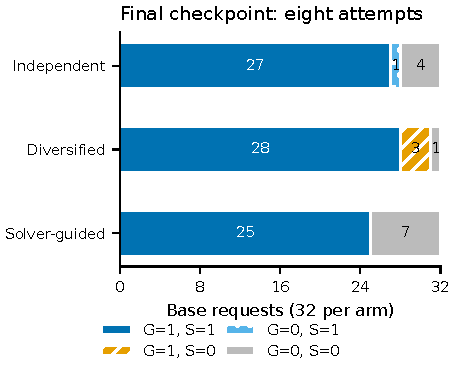
\includegraphics[width=\columnwidth]{figures/joint-outcomes.pdf}
\caption{Study 2 joint outcomes at eight attempts, with 32 requests per arm. $G$ denotes bounded reference-matching candidate availability and $S$ final correctness. Diversified sampling loses three available matching candidates; independent sampling produces one correct plan without one. The off-diagonal cells are computed from request-level records, not inferred from marginal totals. References remain provisional.}
\label{fig:joint}
\end{figure}

Figure~\ref{fig:joint} gives the final joint counts in the order $(1,1),(1,0),(0,1),(0,0)$: independent sampling has $(27,0,1,4)$; diversified sampling $(28,3,0,1)$; solver-guided sampling $(25,0,0,7)$. At four attempts, diversified sampling instead has $(24,1,1,6)$: its equal marginal coverage and correctness of 25 conceal both kinds of off-diagonal outcome. This is why the table must be derived from matched records.

Trace inspection identifies incorrect judgments eliminating the matching candidate in all three diversified final $(1,0)$ cases. Two are false positive judgments and one is a false negative. A fourth such failure occurs at its four-attempt checkpoint. Each final case ends with one surviving class, so an unresolved tie or an unused validation opportunity is not the immediate cause. Truthful witness labels recover the three final cases. Across ordinary Study 2 validation, 11 of 19 distinct cached judgments disagree with provisional references. These are actively selected, difficult witnesses, not a representative judge-accuracy benchmark. In Study 1, the corresponding selected-judgment count is seven disagreements out of 31.

\begin{figure*}[t]
\centering
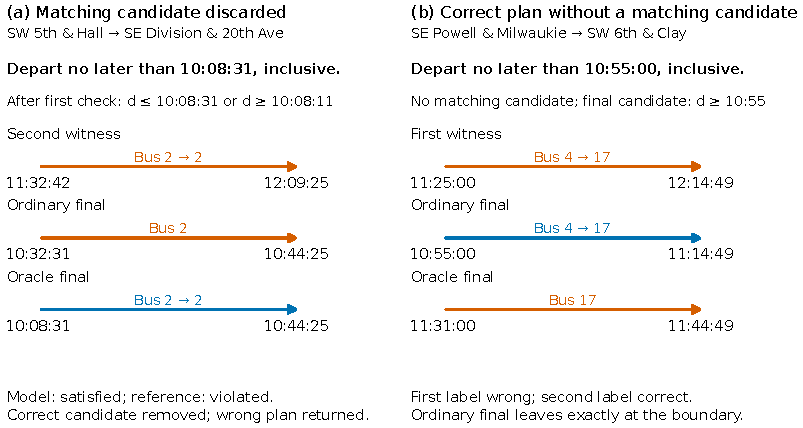
\includegraphics[width=\textwidth]{figures/worked-transit.pdf}
\caption{Illustrative Study 2 cases, selected by the joint cells: the first diversified-sampling $(G=1,S=0)$ case at eight attempts (left), and the sole independent-sampling $(G=0,S=1)$ case there (right). All times are scheduled local service times on 14 September 2026; arrows show journey endpoints, not a time-scaled axis. Left: a false positive on the second witness discards the matching upper-bound candidate. Right: the ordinary path selects a lower-bound formalization whose plan departs exactly at the requested upper bound; truthful first-witness rejection instead leaves an incorrect plan. These examples illustrate mechanisms, not their population prevalence.}
\label{fig:worked}
\end{figure*}

The left example in Figure~\ref{fig:worked} requests departure by 10:08:31. A correct first judgment leaves the matching upper bound and a wrong lower bound. Accepting the second witness, departing 11:32:42, removes the match and yields a 10:32:31 plan. Truthful replay rejects that witness and returns a valid 10:08:31 departure.

\subsection{An Oracle Procedure Is Not a Ceiling}

Oracle-witness replay substitutes reference labels, retaining bounded elimination and the first surviving candidate. It neither inserts candidates nor optimizes reference correctness. Final results are 27/32, 31/32, and 25/32; these happen to equal coverage but measure a different procedure.

Figure~\ref{fig:worked} (right) explains independent sampling's 28 ordinary versus 27 oracle-witness successes. The request requires departure by 10:55; no candidate matches throughout the pool. A wrong positive on an 11:25 departure removes one candidate. A correct second positive retains a lower-bound candidate, whose optimal plan leaves exactly at 10:55 and satisfies the request. Truthful first-witness rejection instead retains a candidate producing an 11:31 departure. Thus truthful labels can change the elimination path and lose a valid decision: this procedure is not an accuracy ceiling.

A separate offline quantity asks whether \emph{any existing candidate's deterministically selected output} is correct. At eight attempts these counts are 28/32, 31/32, and 25/32. This is a best-of-candidate-outputs diagnostic under a precisely restricted output set, not an executable ordinary selector or an unrestricted planning bound. Keeping its meaning separate from $G$ and oracle-witness correctness prevents a misleading claim that ordinary inference exceeded an oracle upper bound.

\subsection{Count Actual Consumption}

Final-prefix logical input/output tokens total 617,643, 626,497, and 811,760 for independent, diversified, and solver-guided sampling across 32 requests each. Solver-guided overhead is 31.43\% and 29.57\%, using the corresponding baseline's consumed generation-plus-validation total as denominator. Logical calls are 266, 269, and 262: fewer calls need not mean fewer tokens.

Across prefixes, counting generation once per trajectory and each prefix's judgments gives 833 logical calls and 2,081,931 tokens. Exact caching reduces actual fresh compute to 659 calls and 1,743,059 tokens. Sampling used 1,207.31 measured GPU-resident seconds plus 53.37 for development and a conservative 60-second allowance. The selector study used 358 calls and 681.62 seconds plus 30 seconds. Shared outputs retain full per-arm logical charges.

\section{\uppercase{Recommendations and Alternatives}}
\label{sec:recommendations}
\noindent Report a linked record per base request: universe and coverage; candidate attempts and signatures; joint availability/correctness; plans, witnesses, judgments, and updates; separate failure categories; and actual/logical cost. Aggregate these records to distinguish opportunity, action, and improvement, rather than replacing correctness with one new score.

Audit benchmark distinctions before candidate availability, then selection and off-diagonal cases, then oracle interventions. One behavioral class offers little basis for comparing example selectors. Losing available alternatives requires a different response from not generating them.

A valid operational decision remains valuable despite a broader specification error, but does not certify future decisions under that formalization. Reporting $G$ alongside $S$ makes this distinction inspectable without turning a successful plan into a semantic certificate.

A small model, weak candidate diversity, or a narrow bus-only universe could explain these outcomes. Stronger or independently trained judges may behave differently. These alternatives limit claims about the interventions, but leave the need to distinguish availability from conversion intact.

Aggregate accuracy remains useful for deployment comparisons. Our concern is explanatory sufficiency: equal totals can conceal different recoverable failures and costs. The independent/diversified comparison has one win and one loss despite identical totals.

Component improvement can matter before final accuracy improves. Diversified sampling supplies more matching candidates, and truthful-witness replay shows a selection opportunity. That is a component finding, not a demonstrated ordinary-pipeline benefit. Shared deterministic time normalization is useful engineering, not a novel sampling mechanism. Repeated lower-bound readings are consistent with feedback anchoring, but do not establish that psychological explanation.

These results warrant pausing expansion of the particular weighting and solver-guided interventions. Neither met its practical objective. Reusable planning and evaluation infrastructure retains value, but theoretical possibility alone does not justify more inference. A future investigation needs a motivated change, fresh data, and its own frozen criterion; inspected requests are not fresh holdout evidence.

\section{\uppercase{Limitations}}
\label{sec:limitations}
\noindent The studies contain 48 and 32 base requests, one model, and one replicate. Constructed wording, overlapping services, and shared translation/judgment models constrain generalization. Data selection and normalization differ across studies; their accuracies must not be pooled. Bootstrap intervals describe these small samples, excluding annotation uncertainty, route dependence, and uncertainty over models and prompts.

Separate reference code reduces implementation dependence; developer checks do not establish independent annotation validity. Systematic wording errors could affect $G$ and $S$ together. No clear correction was found in the selector audit. A worksheet awaits actual author or collaborator review.

The universe is not the full network. Conditional infeasibility is weaker than real-world impossibility. The subset excludes available non-bus services; transfer clauses can be vacuous, visit clauses do not independently test order, and daytime requests do not test midnight or daylight saving. Study 2's stronger clause checks improve informativeness without broadening these claims.

Matching signatures can conceal semantic differences lacking counterexamples. Clause-level signatures expose variation masked by a rejecting conjunct, but source-clause associations are not always available. This framework therefore measures bounded behavior, not unrestricted source fidelity; selected-witness disagreements are not general judge error rates.

The position arose from exploratory findings, not a preregistered reporting hypothesis. Its components have substantial precedents, and the combined procedure is not validated as a universal standard. These cases illustrate diagnostic value, not that the procedure itself improves models or that the interventions fail elsewhere.

\section{\uppercase{Conclusion}}
\label{sec:conclusion}
\noindent Plan correctness, matching-candidate availability, and benchmark informativeness are different properties. Here weighting rarely changed behavior, diversified sampling improved coverage without improving final correctness, and solver-guided sampling added cost without useful coverage. Joint outcomes and defined oracle interventions explain these findings better than marginal accuracy alone. Evaluate the path from tested requirements to available interpretations to selected decisions, and report where it breaks.

\subsection*{AI Assistance Disclosure}
\label{sec:ai}
OpenAI Codex \cite{codex} assisted prose throughout, offline analysis/plotting code, and artifact checks. Underlying requests and implementation also used AI assistance. Numbers derive from saved outputs, with no new experimental inference. Figures use deterministic plotting, not image generation. References lack independent human adjudication. Submitting authors remain responsible for the content and final declarations.

\begin{thebibliography}{99}
\bibitem[Amonkar et~al., 2026]{amonkar}
Amonkar, R., Kayan, C.~E., Lai, Q., Le~Bras, R., and Zhang, L. (2026).
A reality check of language models as formalizers on constraint satisfaction problems.
\emph{arXiv:2505.13252v6}. Preprint; first submitted 2025.
\href{https://arxiv.org/abs/2505.13252v6}{doi:10.48550/arXiv.2505.13252}.

\bibitem[GTFS, 2026]{gtfs}
GTFS (2026). Schedule reference.
\url{https://gtfs.org/documentation/schedule/reference/}. Accessed 13 September 2026.

\bibitem[Mendoza et~al., 2026]{artemis}
Mendoza, D., Mavridou, A., Katis, A., and Trippel, C. (2026).
Automating requirements formalization: Using LLMs and low-complexity distinguishing traces for semantic validation.
In \emph{48th IEEE/ACM International Conference on Software Engineering (ICSE)}.
\href{https://doi.org/10.1145/3744916.3787815}{doi:10.1145/3744916.3787815}.

\bibitem[OpenAI, 2026]{codex}
OpenAI (2026). Codex. AI assistance tool.
\url{https://openai.com/codex/}. Accessed 13 September 2026.

\bibitem[Qwen Team, 2024]{qwen}
Qwen Team (2024). Qwen2.5-7B-Instruct: Official model card.
\url{https://huggingface.co/Qwen/Qwen2.5-7B-Instruct}. Accessed 13 September 2026.

\bibitem[Raza and Milic-Frayling, 2025]{ssv}
Raza, M. and Milic-Frayling, N. (2025).
Instantiation-based formalization of logical reasoning tasks using language models and logical solvers.
In \emph{Proceedings of IJCAI-25}, pages 4633--4641.
\href{https://doi.org/10.24963/ijcai.2025/516}{doi:10.24963/ijcai.2025/516}.

\bibitem[Singh et~al., 2026]{verge}
Singh, V., Cassel, D., Weir, N., Feng, N., and Bayless, S. (2026).
VERGE: Formal refinement and guidance engine for verifiable LLM reasoning.
\emph{arXiv:2601.20055v2}. Preprint.
\href{https://arxiv.org/abs/2601.20055v2}{doi:10.48550/arXiv.2601.20055}.

\bibitem[TriMet, 2026]{trimet}
TriMet (2026). GTFS schedule data.
\url{https://developer.trimet.org/GTFS.shtml}. Feed version 20260823-20260910-0900; acquired September 2026.

\bibitem[Wang et~al., 2026]{diversity}
Wang, T., Liu, Z., Chen, Y., Light, J., Liu, W., Chen, H., Zhang, X., and Cheng, W. (2026).
On the effect of sampling diversity in scaling LLM inference.
\emph{arXiv:2502.11027v5}. Preprint; first submitted 2025.
\href{https://arxiv.org/abs/2502.11027v5}{doi:10.48550/arXiv.2502.11027}.
\end{thebibliography}
\end{document}
